\section{Continuum-Mechanical Model of the Upper Limb}
\label{sec:71model}

\minitoc{71mm}{5}

\noindent
In the following, we first discuss the state of the art
in biomechanical modeling.
Then, we address the details of the model of the human upper limb
such as its parameters and its geometry.
For convenience, the most relevant symbols that occur
in the context of biomechanical models are listed in
\cref{tbl:glossaryBiomechanical}.

\begin{table}
  \setnumberoftableheaderrows{0}%
  \newcommand*{\pnst}[1]{\printnotationsymbol{#1}&\printnotationtext{#1}}%
  \begin{tabular}{%
      >{\kern\tabcolsep}=l+l<{\kern5mm}+l+l<{\kern5mm}+l+l<{\kern\tabcolsep}%
    }
    \toprulec
    \pnst{\forcetriceps}& \pnst{\armtriceps}& \pnst{\elbowangle}\\
    \pnst{\forcebiceps}&  \pnst{\armbiceps}&  &\\
    \pnst{\forceload}&    \pnst{\armload}&    &\\
    \bottomrulec
  \end{tabular}%
  \caption[Glossary for biomechanical models]{%
    Glossary of the notation for biomechanical models.%
  }%
  \label{tbl:glossaryBiomechanical}%
\end{table}



\subsection{Continuum-Mechanical Musculoskeletal Models}
\label{sec:711models}

\paragraph{Limitations of lumped-parameter models}

Due to the simplicity and computational efficiency of
classical lumped-parameter models,
their degree of realism is limited.
Without any modifications,
lumped-parameter models are not able to represent
detailed heterogeneous material characteristics or non-trivial
muscle force paths \cite{Roehrle16Two}.

\paragraph{Benefits of continuum-mechanical models}

The exploitation of continuum-mechani\-cal constitutive laws
for musculoskeletal models is a more recent development \cite{Roehrle16Two}.
The resulting models are capable to model spatial quantities
such as complex muscle fiber field architectures,
local activation principles, complex muscle geometries, or contact mechanics
\multicite{Roehrle16Two,Valentin18Gradient}.
Most of existing work only treats a single skeletal muscle in isolation
\multicite{Lemos05Modeling,Sharafi11Strains,Heidlauf14Multiscale}.
The goal of the model used in this thesis
(which is the same model as in
\multicite{Sprenger15Continuum,Roehrle16Two,Valentin18Gradient})
is to study the interplay of multiple muscles and bones.

\paragraph{Overdetermined antagonistic systems}

Musculoskeletal systems are typically overdetermined \cite{Roehrle16Two}.
This means that the number of muscles that act on a specific joint
is usually larger than the number of the joint's degrees of freedom.
For instance, in a simple model of the upper limb,
there are two antagonistic muscles
(i.e., muscles that work against each other), namely biceps and triceps,
but only one joint angle at the elbow.
Mathematically speaking, a single muscle would suffice to attain
most elbow angles that are possible with an antagonistic muscle pair.
However, the usage of two muscles enables faster movements and
allows for abrupt changes of direction.

The overdetermination of most musculoskeletal models
implies that additional conditions have to be imposed in order
to obtain unique solutions.
There exist various types of such conditions,
for instance, minimal control effort, minimal control change, and
minimal kinematic energy \cite{Valentin18Gradient}.
The idea behind all of these conditions is that the human body
tries to minimize the energy effort that is associated with
most types of motion.

\paragraph{Forward and inverse dynamics}

Musculoskeletal simulations are usually based on
either forward dynamics or inverse dynamics \cite{Valentin18Gradient}.
\term{Forward-dynamic approaches} use activation parameters
for the muscles as the input and simulate the corresponding motion
as the output.
This requires that we know the muscle forces beforehand,
depending on the activation levels.
For example, one can prescribe activation levels of facials muscles
to achieve specific facial expressions \cite{Wu13Modelling}.
In contrast, \term{inverse-dynamic approaches}
use experimental motion data as the input
to estimate the muscle forces as the output \cite{Roehrle16Two}.
With inverse-dynamic simulations,
one can investigate the wrapping of muscles
around the knee joint \cite{Fernandez05Anatomically} or
visualize the motion of skin \cite{Lee09Comprehensive}, for instance.



\subsection{Details of the Human Upper Limb Model}
\label{sec:712details}

\begin{figure}
  \raisebox{-\height}{\rlap{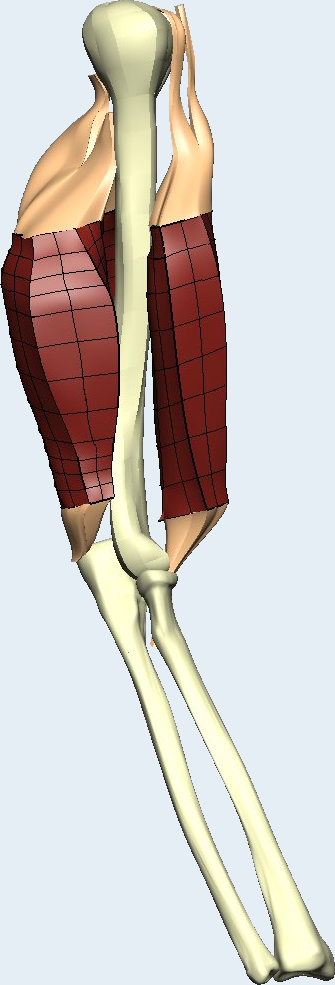
\includegraphics[scale=0.13]{upperLimb_1}}}%
  \hfill%
  \raisebox{-\height}{\rlap{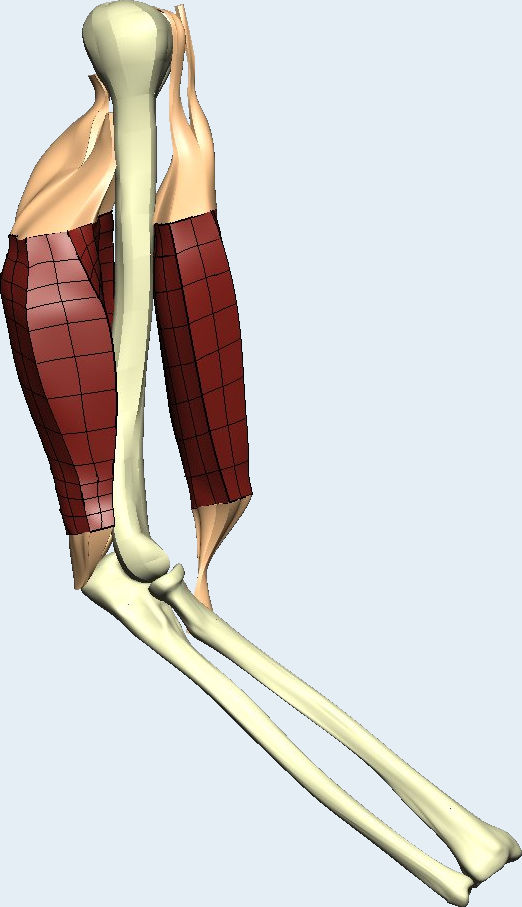
\includegraphics[scale=0.13]{upperLimb_2}}}%
  \hfill%
  \raisebox{-\height}{\rlap{\includegraphics[scale=0.13]{upperLimb_3}}}%
  \hfill%
  \raisebox{-\height}{\rlap{\includegraphics[scale=0.13]{upperLimb_4}}}%
  \hfill%
  \raisebox{-\height}{\rlap{\includegraphics[scale=0.13]{upperLimb_5}}}%
  \hfill\strut%
  \caption[Raising arm movement]{%
    Human upper limb model geometry shown as raising arm movement
    for the elbow angles
    \SI{10}{\degree}, \SI{45}{\degree}, \SI{80}{\degree},
    \SI{115}{\degree}, and \SI{150}{\degree} \emph{(from left to right).}
    Taken from \cite{Sprenger15Continuum}.%
  }%
  \label{fig:raisingArm}%
\end{figure}

\paragraph{Overall stress}

\cite{Soennerlind13Why}

\dummytext{}

\paragraph{Parameters and geometry}

\cite{Spitzer96Visible}
\cite{Sprenger15Continuum}

\dummytext{}
